% !TEX encoding = UTF-8 Unicode

\documentclass[a4paper]{article}

\usepackage{color}
\usepackage{url}
\usepackage[T2A]{fontenc} % enable Cyrillic fonts
\usepackage[utf8]{inputenc} % make weird characters work
\usepackage{graphicx}

\usepackage[english,serbian]{babel}

\usepackage[unicode]{hyperref}
\hypersetup{colorlinks,citecolor=green,filecolor=green,linkcolor=blue,urlcolor=blue}

\newtheorem{primer}{Primer}[section]

\DeclareUnicodeCharacter{0301}{\'{c}}

\title{Roboti kao nastavnici\small \\Seminarski rad u okviru kursa\\Tehničko i naučno pisanje\\Matematički fakultet}
\author{Jovan Mijajlović, jovan.mijajlovic03@gmail.com\\Miona Sretenović, sretenovicmiona7@gmail.com\\Mina Protić, minaproticc@gmail.com\\Mihailo Marković, mihailoo003@gmail.com}
\date{11.~novembar 2022}

\begin{document}
\maketitle
\tableofcontents
\newpage

\section{Uvod}

Roboti stižu u školske klupe!
Roboti, kao pomoć nastavnicima informatike, stižu u školske klupe. Đaci će se po prvi put uveriti da programiranje nije apstraktno, jer će ono što su isprogramirali izvršavati roboti. Dosad se za tu obuku prijavilo više od 400 nastavnika, a plan je da svi nastavnici informatike budu uključeni, ali i da svaka škola dobije po pet robota. Međutim, postavlja se pitanje koliko je to izvodljivo?
Da bismo govorili o ovoj temi moramo se prvo upoznati sa time šta su roboti a šta nastavnici.

\section{Šta su roboti?}
Robot jeste elektro-mehanička jedinica koja je u stanju da autonomno, po nekom programu, ili pod kontrolom čoveka izvodi određene zadatke. Roboti se koriste za izvođenje zadataka opasnih, teških ili napornih za ljude. Na primer sakupljanje nuklearnog otpada ili slaganje velikog broja žica prema boji, kao i repetitivne poslove gde se zahteva istrajnost i preciznost, kao što je sklapanje motora i šasije automobile.
Roboti koji imaju oblik ljudskog tela se još zovu humanoidni roboti. Ako je uz ovo još i svrha da se po njihovim ostalim karakteristikama, kao što su kretanje, govor, gestikulacije itd, što više približe ljudskim bićima, radi se o androidima. Ovaj termin se ipak češće sreće u naučnoj fantastici.
Inteligenciju koju robot poseduje čini u stvari program ili sistem programa, koji određuje sposobnost robota da prepozna određene situacije i da se u njima snađe ili ih rešava, ponašajući se na pravi način ili čak iz sopstvenog iskustva uči kako da se snalazi u novim situacijama i rešava nove probleme. Ova vrsta inteligencije se zove još i veštačka inteligencija i predstavlja zasebnu granu nauke. Izraz „robot“ se prvi put pominje u drami čehoslovačkoga pisca Karela Čapeka „R. U. R.“. Za termin robot zaslužan je njegov brat Josef Čapek. Reč je nastala na čehoslovačkom jeziku pa se onda proširila na ceo svet.
Roboti mogu da budu autonomni ili poluautonomni i u opsegu su od humanoidnih kao što je Hondin Napredni korak u inovativnoj mobilnosti (ASIMO) i TOSY-jev TOSY robot koji igra ping pong (TOPIO) do industrijskih robota, medicinskih operativnih robota, onih koji pomažu pacijentima, robota za pseću terapiju, kolektivno programiranih rojskih robota, bespilotnih letelica kao što je MQ-1 predator, i mikroskopskih nano robota. Putem oponašanja izgleda živih bića ili automacije pokreta, robot može da pruži osećaj inteligencije ili sopstvenog razmišljanja. Očekuje se da će doći do proliferacije autonomnih predmeta u narednim dekadama, pri čemu su kućna robotika i autonomna kola među vodećim oblastima primene.


\begin{figure}[h!]
\begin{center}
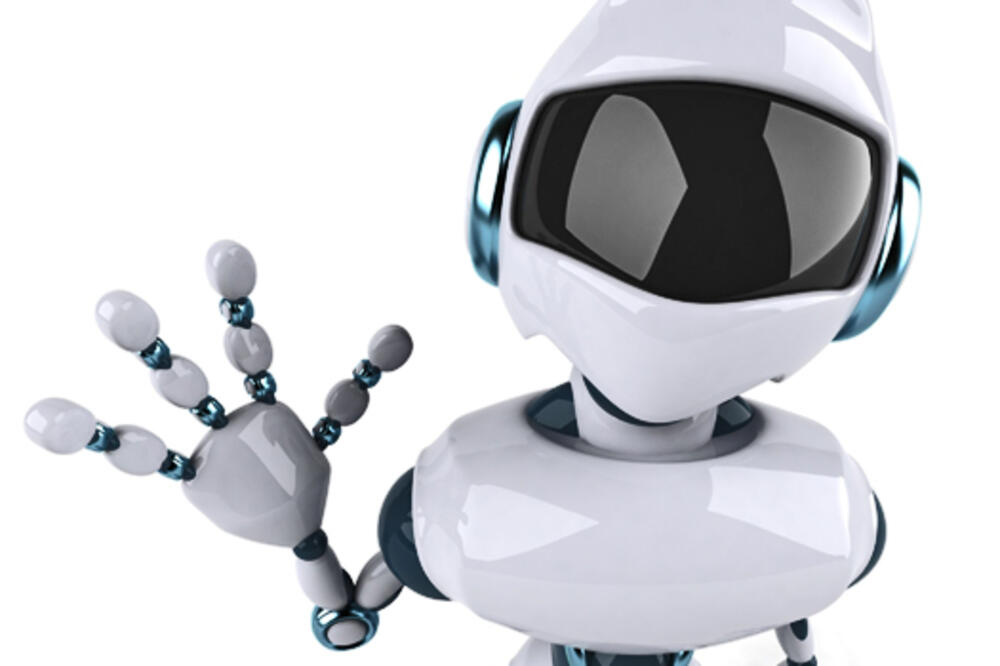
\includegraphics[scale=0.3]{robotm.jpg}
\caption{Robot}
\end{center}
\label{fig:robot}
\end{figure}

\newpage
\section{Šta su nastavnici?}
Nastavnik je stručna osoba visokih radnih, obrazovnih i etičkih kvaliteta edukovana za rad u vrtiću, školi ili fakultetu za određen predmet. On mora da zadovolji niz specifičnih zahteva kao što su: svesna motiviranost za zvanje, potpuniji sastav opšteg i stručnog obrazovanja, visoke intelektualne sposobnosti, crte ličnosti adekvatne sastavu vrednosti u društvu, visoki nivo zrelosti ličnosti, kao i visoki nivo lične kulture.

\begin{figure}[h!]
\begin{center}
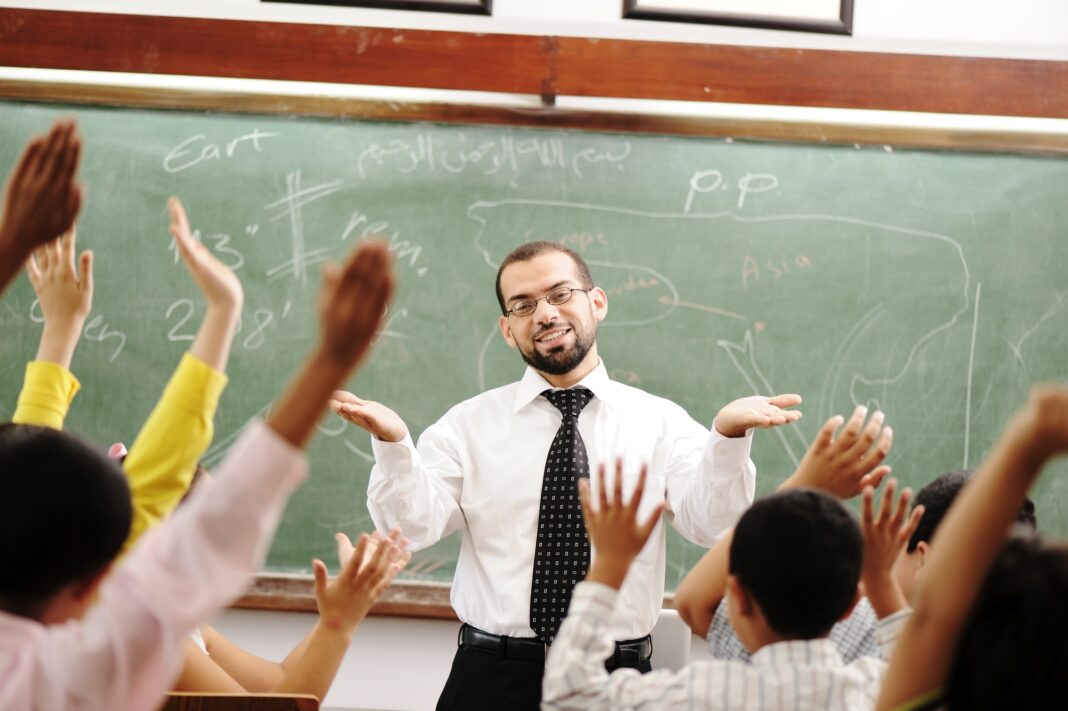
\includegraphics[scale=1.2]{nastavnik.jpg}
\caption{Nastavnik}
\end{center}
\label{fig:nastavnik}
\end{figure}

\newpage
\subsection{Entuzijazam nastavnika}
Utvrđeno je da nastavnici koji su pokazali entuzijazam prema materijalima kursa i studentima mogu stvoriti pozitivno iskustvo učenja. Ovi nastavnici ne predaju napamet, već pokušavaju da osnaže svoje predavanje materijima kursa svakog dana. Nastavnicima koji ponavljaju isti nastavni plan i program može biti izazov da održe svoj entuzijazam, kako se njihova dosada sa sadržajem ne bi negativno odražavala na njihove učenike. Nastavnike entuzijaste njihovi učenici ocenjuju više od nastavnika koji nisu pokazali mnogo entuzijazma za materijale kursa.
Nastavnici koji pokazuju entuzijazam imaju veću verovatnoću da imaju angažovane, zainteresovane i energične učenike koji su radoznali da nauče predmet. Nedavno istraživanje je otkrilo korelaciju između entuzijazma nastavnika i unutrašnje motivacije učenika da uče i vitalnosti u učionici. Kontrolisane, eksperimentalne studije koje istražuju intrinzičnu motivaciju studenata pokazale su da neverbalni izrazi entuzijazma, kao što su demonstrativna gestikulacija, dramatični pokreti koji su različiti i emocionalni izrazi lica, dovode do toga da studenti prijavljuju više nivoe unutrašnje motivacije za učenje. Ali čak i ako se pokazalo da entuzijazam nastavnika poboljšava motivaciju i povećava angažovanje u zadatku, to ne mora nužno da poboljša ishode učenja ili pamćenje materijala.
Postoje različiti mehanizmi pomoću kojih entuzijazam nastavnika može olakšati viši nivo unutrašnje motivacije. Entuzijazam nastavnika može doprineti atmosferi energije i entuzijazma u učionici koja podstiče interesovanje i uzbuđenje učenika u učenju predmeta. Nastavnici entuzijasti mogu takođe dovesti do toga da učenici postanu samoopredeljeni u sopstvenom procesu učenja. Koncept pukog izlaganja ukazuje na to da nastavnikov entuzijazam može doprineti očekivanjima učenika o intrinzičnoj motivaciji u kontekstu učenja. Takođe, entuzijazam može delovati kao „motivaciono ulepšavanje“, povećavajući interesovanje učenika raznovrsnošću, novinom i iznenađenjem entuzijastičnog nastavnika koji predstavlja materijal. Konačno, može se primeniti i koncept emocionalne zaraze: učenici mogu postati suštinski motivisani uhvaćenim entuzijazmom i energijom nastavnika.

\subsection{Interakcija nastavnika sa učenicima}
Istraživanja pokazuju da su motivacija učenika i stavovi prema školi usko povezani sa odnosima učenika i nastavnika. Nastavnici entuzijasti su posebno dobri u stvaranju korisnih odnosa sa svojim učenicima. Njihova sposobnost da stvore efektivno okruženje za učenje koje podstiče postignuća učenika zavisi od vrste odnosa koji grade sa svojim učenicima. Korisne interakcije između nastavnika i učenika su ključne za povezivanje akademskog uspeha sa ličnim dostignućima. Ovde je lični uspeh unutrašnji cilj učenika da se unapredi, dok akademski uspeh uključuje ciljeve koje dobija od svog pretpostavljenog. Nastavnik mora da vodi svog učenika u usklađivanju svojih ličnih ciljeva sa njihovim akademskim ciljevima. Učenici koji prime ovaj pozitivan uticaj pokazuju jače samopouzdanje i veći lični i akademski uspeh od onih bez ovih interakcija sa nastavnicima.
Učenici će verovatno izgraditi jače odnose sa nastavnicima koji su prijateljski raspoloženi i podržavaju ih i pokazaće više interesovanja za kurseve koje predaju ovi nastavnici. Nastavnici koji provode više vremena u interakciji i direktnom radu sa učenicima smatraju se efikasnim nastavnicima koji pružaju podršku. Pokazalo se da efikasni nastavnici pozivaju učenike na učešće i donošenje odluka, dozvoljavaju humor u svojoj učionici i pokazuju spremnost za igru.

Stvari koje se traze od nastavnika:
\begin{itemize}
\item{} Znanje (kao što su: sam predmet i znanje o tome kako ga predavati, znanja iz nastavnog plana i programa, znanja o obrazovnim naukama, psihologija, ocenjivanje itd.);
\item{} Zanatske veštine (kao što su planiranje časa, korišćenje nastavnih tehnologija, upravljanje učenicima i grupama, praćenje i procena učenja, itd.);
\item{} Dispozicije (kao što su suštinske vrednosti i stavovi, uverenja i posvećenost).
\end{itemize}

\section{Roboti kao nastavnici}
Moramo se zapitati da li roboti mogu da ispune ove kriterijume I da li mogu da zamene čoveka u nastavi?

Britanski stručnjak za obrazovanje Entoni Seldon misli da mogu. Čak ima i datum za robotsko preuzimanje učionice: 2027. On predviđa da će roboti obavljati glavni posao prenosa informacija i da će nastavnici biti kao asistenti. Inteligentni roboti će čitati lica učenika, pokrete i možda čak i moždane signale. Zatim će informacije prilagoditi svakom učeniku. To nije popularno mišljenje i malo je verovatno da će roboti ikada imati empatiju i sposobnost da se stvarno povežu sa ljudima kao što drugi ljudi mogu.
Jedno je ipak sigurno. Učitelj robota je bolji nego nikakav učitelj. U nekim delovima sveta nema dovoljno nastavnika i 9–16 odsto dece mlađe od 14 godina ne ide u školu. Taj problem bi delimično mogli da reše roboti jer mogu da predaju bilo gde i neće biti pod stresom, ili umorni, niti se presele negde radi lakšeg, bolje plaćenog posla.
Ti negativni aspekti podučavanja su nešto oko čega se svi slažu. Nastavnici širom sveta odlaze jer je to težak posao i osećaju se prezaposleno. Možda pitanje nije 'Da li će roboti zameniti nastavnike?' ali 'Kako roboti mogu pomoći nastavnicima?' Kancelarijski radnici mogu da koriste softver da rade stvari kao što su organizovanje i odgovaranje na e-poštu, organizovanje sastanaka i ažuriranje kalendara. Nastavnici gube mnogo vremena radeći nenastavne poslove, uključujući više od 11 sati nedeljno obeležavajući domaći zadatak. Kada bi roboti mogli da smanje vreme koje nastavnici troše na obeležavanje domaćih zadataka i pisanje izveštaja, nastavnici bi imali više vremena i energije za delove posla koji ljudi najbolje obavljaju.
\end{document}
